% ================= FRONT MATTER =================
\frontmatter
\pagestyle{empty}
% ---- half-title (i) ----
\vspace*{1.9in}
\begin{center}
\lsc{\large an ideological offensive}\\[0.5ex]
\lsc{\large for the free world}
\end{center}
\cleartoverso
% ---- (ii) blank ----
\null
\cleartorecto
% ---- title page (iii) ----
\begin{center}
\vspace*{0.85in}
{\Huge\textls[30]{\scshape An Ideological}\par}\vspace{0.35\onelineskip}
{\Huge\textls[30]{\scshape Offensive}\par}\vspace{0.35\onelineskip}
{\Large\itshape for the\par}\vspace{0.35\onelineskip}
{\Huge\textls[30]{\scshape Free World}\par}
\vspace{1.4\onelineskip}
\rule{3em}{0.4pt}
\vspace{1.4\onelineskip}

{\large\itshape by\par}\vspace{0.6\onelineskip}
{\Large\lsc{Colonel John J. Fischer}\par}\vspace{0.3\onelineskip}
{\itshape United States Air Force\par}

\vfill
{\small\itshape An Individual Research Paper\par}
{\small\lsc{the national war college}\par}
{\small Washington, D.\,C.\,\textperiodcentered\, 1 March 1957\par}
\vspace{2.2\onelineskip}
{\footnotesize\lsc{family edition}\enspace\textperiodcentered\enspace 2026\par}
\vspace*{0.1in}
\end{center}
\clearpage
% ---- copyright page (iv) ----
{\footnotesize\setlength{\parindent}{0pt}\setlength{\parskip}{0.55\onelineskip}
\vspace*{\fill}
\textit{An Ideological Offensive for the Free World}\\
by Colonel John J. Fischer, United States Air Force

Written as an Individual Research Paper at The National War College, Washington, D.\,C., and dated 1 March 1957.

Family edition, privately printed in 2026 for the family of John~J. Fischer. Not for sale.

This work was prepared by a serving officer of the United States Air Force as part of his course of study at The National War College. As a work of the United States Government it is believed to be in the public domain in the United States (17~U.S.C. §\,105). The original typescript bore the College’s 1957 restriction on quotation and reproduction, which is preserved in the facsimile of its title page in this edition, together with the following statement:

\textit{The opinions and conclusions expressed herein are those of the individual student author and do not necessarily represent the views of either the National War College or any other governmental agency.}

Transcribed from the original 121-page typescript. See the Note on the Transcription.

Set in EB Garamond.

Printed in the United States of America.
\par}
\cleartorecto
% ---- dedication (v) ----
\vspace*{2.2in}
\begin{center}
{\footnotesize\lsc{[draft]}\par}\vspace{0.8\onelineskip}
\itshape For the children, grandchildren and great-grandchildren\\
of John J. Fischer,\\[0.5ex]
[placeholder dedication]
\end{center}
\cleartorecto
\pagestyle{fischer}
% ---- contents ----
{\setlength{\beforechapskip}{0.35in}\tableofcontents*}
\cleartorecto
% ---- family foreword ----
\chapter{Foreword}
\begin{center}\footnotesize\lsc{[draft --- placeholder text]}\end{center}
\vspace{0.5\onelineskip}

\noindent\textsc{[In 1957]} Colonel John J. Fischer of the United States Air Force was a student at The National War College in Washington. [A few paragraphs from the family will go here: who he was, his service, how the typescript came down through the family, and why it has been set in type now.]

[Second paragraph: the world of 1957 --- Sputnik was months away, the Hungarian revolution only just crushed --- and what this paper shows of the man who wrote it.]

[Closing paragraph and acknowledgments.]

\vspace{1.2\onelineskip}
\begin{flushright}\itshape [Name]\\ Brooklyn, New York, 2026\end{flushright}

% ---- note on the transcription ----
\chapter{A Note on the Transcription}

\noindent\textsc{This edition} reproduces the text of the original typescript of March 1957, 121 pages, from a careful transcription checked line by line against images of every page. The author’s wording, spelling and punctuation have been kept, including the usages of his day (\textit{indorsed}, \textit{thru}, \textit{benefitted}). Words divided at the ends of typed lines have been closed up, and the few letters blurred on the old paper have been read from context; otherwise the text stands as it was typed.

The typescript gathered its 142 notes at the end of the paper, keyed to the text by numbers in the form “1/”. Here they are set as footnotes at the foot of the page. They are numbered consecutively; in Chapter~IV three notes were typed out of sequence (59, 60, 61), and they are numbered here in reading order, each still attached to its original reference. The notes to the sections on Adam Smith and on Malthus and Ricardo were keyed to those headings in the typescript, and are so placed here.

Underlining in the typescript is shown in italics. Where the author quotes a source and types some of its words in capitals---the typist’s way of reproducing the source’s own italics---those words are set here in italics, as the source printed them (in roman where the surrounding passage is itself italic); the author’s own emphasis within a quotation is marked, as in the original, “(underscoring supplied).” The marginal notes that accompany the long extract from the \textit{Communist Manifesto} in Chapter~III are given in small italic type before the passages they gloss.

The typescript’s running headers, page numbers and table of contents have not been reproduced; the chapter and section titles are the author’s. His title page, with the restriction notice that governed the paper’s circulation in 1957, is reproduced in facsimile opposite.

% ---- facsimile on the verso facing the Preface ----
\cleartoverso
\thispagestyle{empty}
\vspace*{\fill}
\begin{center}
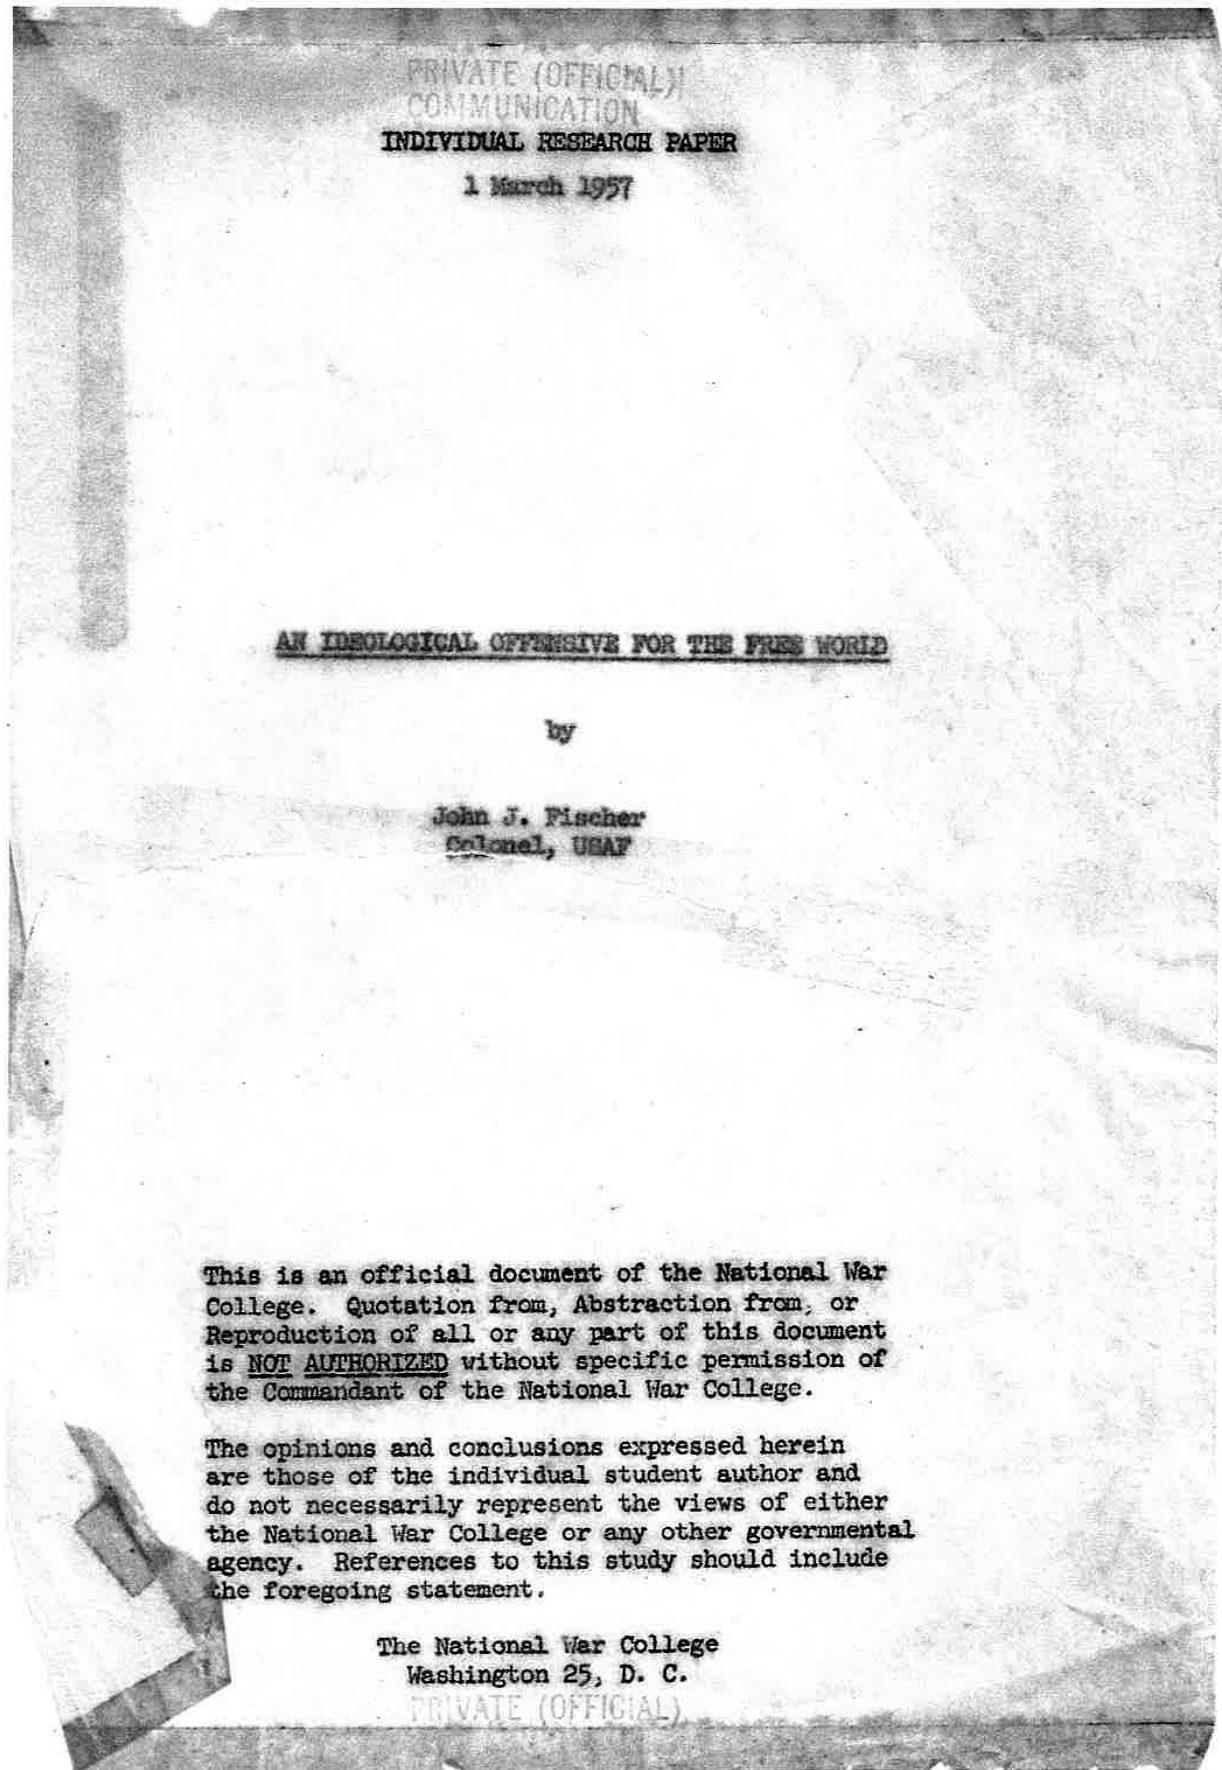
\includegraphics[width=0.94\textwidth,height=0.86\textheight,keepaspectratio]{img/facsimile-title.png}\par
\vspace{0.8\onelineskip}
{\footnotesize\itshape The title page of the original typescript, 1957.\par}
\end{center}
\vspace*{\fill}
\clearpage
